\section{Method}
In this section, we first illustrate the problem definition of \taskfullname~(\taskabbrname). 
Then we elaborate on the model architecture and training process.

\begin{figure*}[ht!]
    \centering
    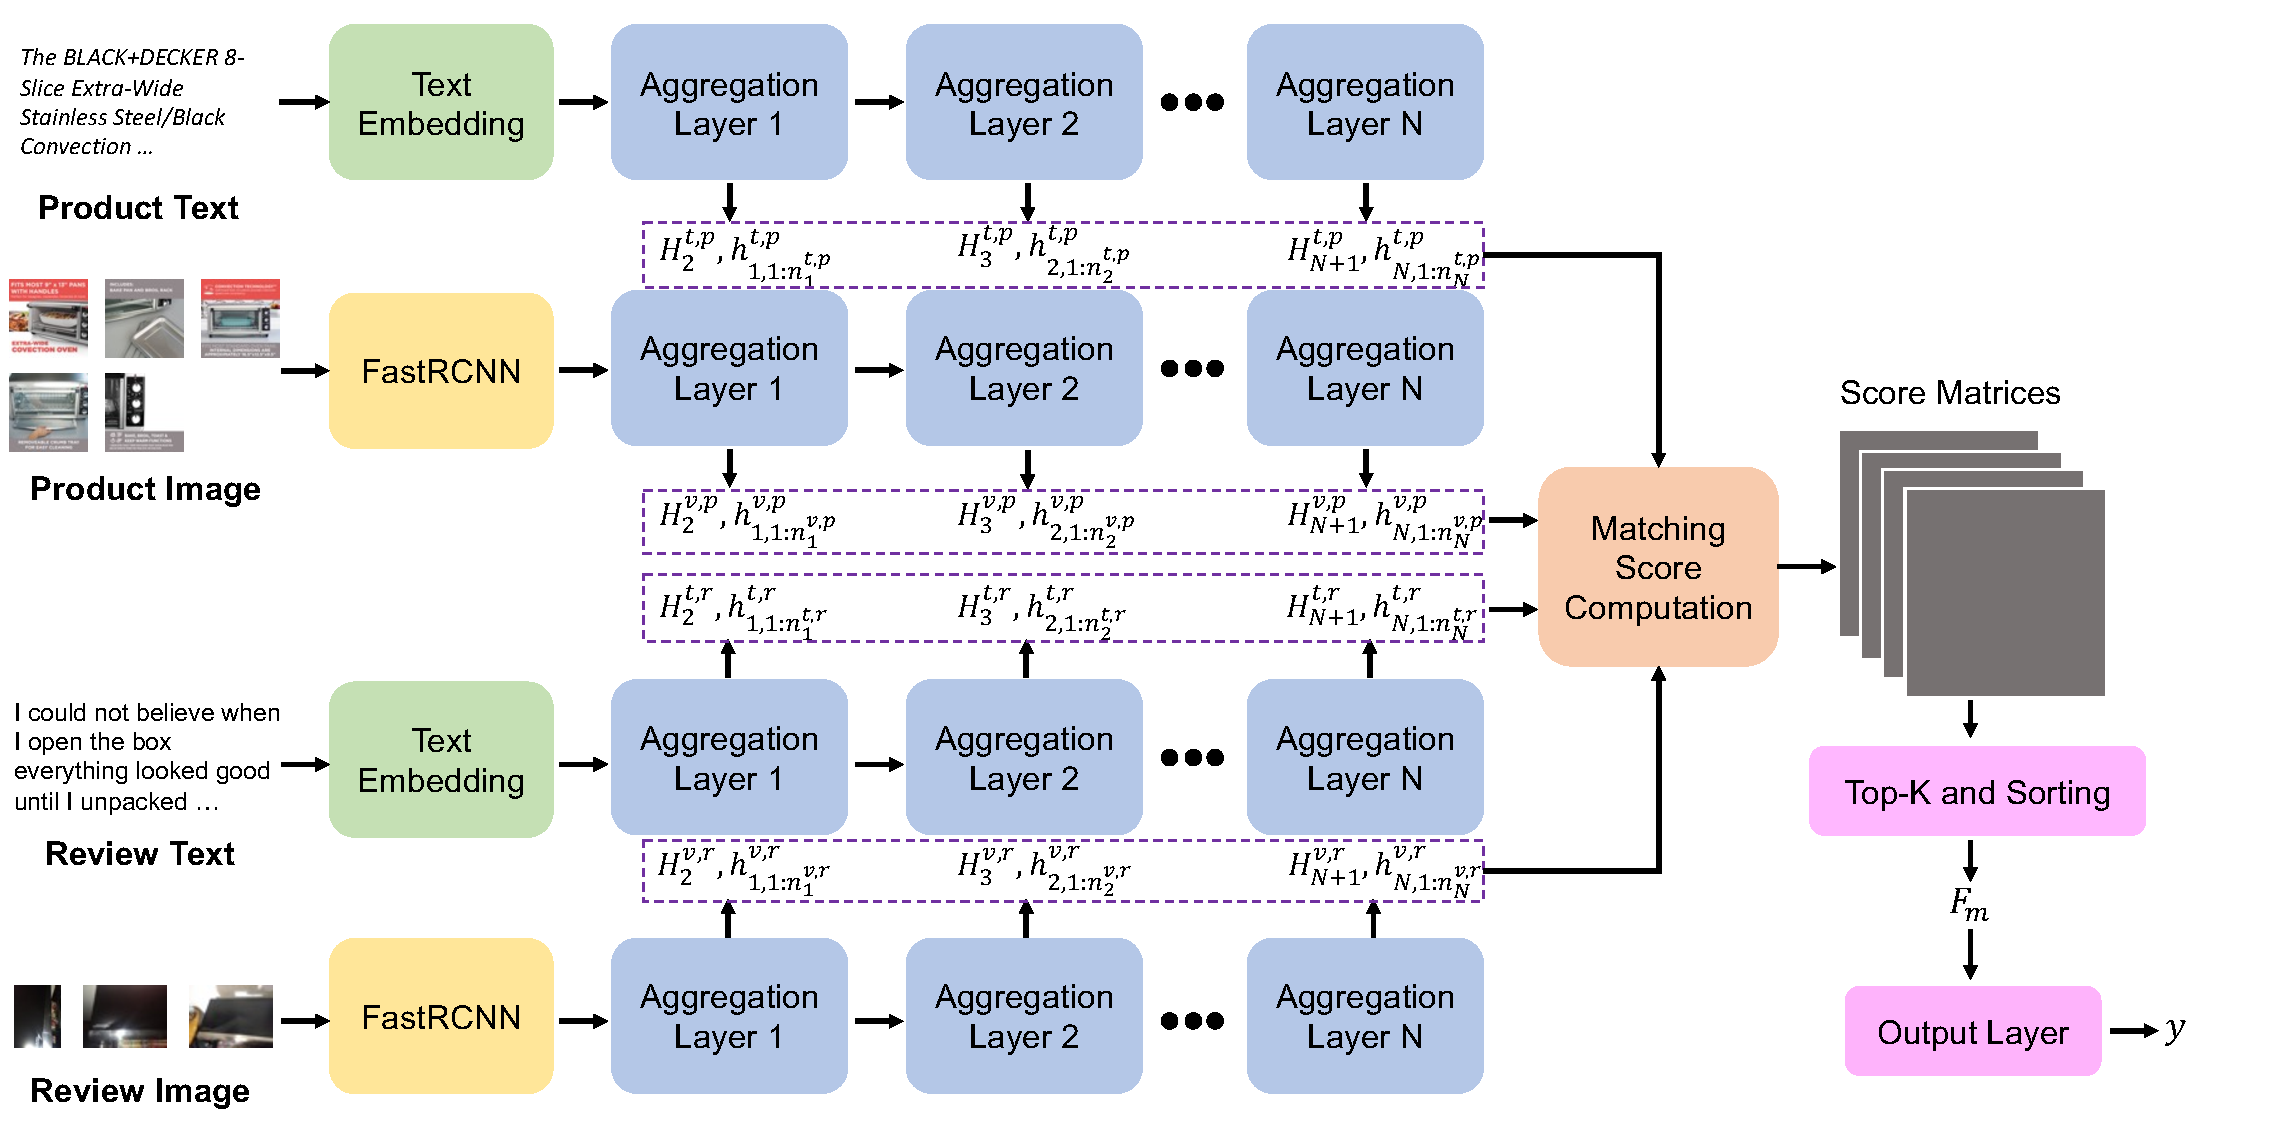
\includegraphics[trim=0.5cm 0.5cm 2cm 2cm, width=0.92\textwidth]{Contents/img/Model.pdf}
    \caption{The overall architecture of~\modelname. We hide the data frame reorganization process betwixt two aggregation layers that merge the produced larger-scale representations into a new sequence and only show the outputs from a single block of data with the subscript $i$ omitted for simplicity.}
    \label{model}
\end{figure*}

\subsection{Problem Definition}
Given $N$ product descriptions $\mathcal{P}=\{P_1,P_2,...,P_N\}$ and their associated review sets $\mathcal{R}=\{R_1,R_2,...,R_N\}$, where the review set $R_i$ contains $m_i$ pieces of review $R_i=\{r_{i,1},r_{i,2},...,r_{i,m_i}\}$. 
Both the product descriptions and review pieces
% (termed \textit{fields} below) 
are presented in the modality of text $T_{p_i/r_{i,k}}$ and image $I_{p_i/r_{i,k}}$. 
MRHP aims to predict the helpfulness scores of reviews $\{y_{i,k}\}_{k=1}^{m_i}$ and rank these reviews according to the scores in descending order so that favorable reviews can be promoted to the top.
For the simplicity of the statement, we call the product description and review \textit{field}, denoted by the superscripts $f\in\{p,r\}$. 
Similarly the superscripts $m\in\{t,v\}$ refer to the \textit{modality} of text and image (vision). 

\subsection{Overview}
We depict the overall architecture of our model in~\Cref{model}. 
At the bottom layer, the modality-specific encoders are pretrained models or word vectors that map the raw inputs into continuous embeddings.
The initially embedded representations are viewed as the minimal scale to be aggregated by~\modelname. 
For example, they are word vectors if the encoder is Glove~\cite{pennington2014glove}, contextualized word representations if applying BERT~\cite{devlin2018bert} or other pretrained language models, and detected hot regions in an image when adopting FastRCNN~\cite{Girshick_2015_ICCV}.
These representations are then passed through $N$ stacked aggregation layers where representations from a smaller scale are collated into larger-scale counterparts.
Finally,~\modelname~computes the matching scores between these multi-scale feature vectors and performs regression with the sorted top-K scores.

\subsection{Input Feature}
\paragraph{Textual Representation}
We initialize the token representations of text in the product and review fields with word vectors or pretrained models as
$\mathbf{E'}_t = \{e_1^{'t}, e_2^{'t}, ..., e_l^{'t}\} $, where $l$ is the length of a review sentence. 
For word vector embeddings, we additionally exploit a Gated Recurrent Unit (GRU) \citep{cho2014learning} layer on each sentence to obtain the context-aware token-level representations $\mathbf{E}_t= \{e_1^t, e_2^t, ..., e_l^t\}$,
where $\theta_t$ denotes the parameters of the GRU.

\paragraph{Visual Representation} 
We embed images with pretrained Faster R-CNN \citep{ren2015faster}, which utilizes ResNet-101 as its backbone, yieding the visual feature input $\mathbf{E}_v=\{e_1^v,e_2^v,...,e_{n_h}^v\}$.
where $\theta_v$ denotes the parameters in FastRCNN and $n_h$ is the number of hot regions detected in the given image.

% \subsection{Disparity Maximization}

\subsection{Multi-Scale Matching Network (MSMN)}
The inspiration beneath MSMN is from the pyramid and network-in-network architectures~\cite{lazebnik2006beyond,han2021transformer} and relation-based learning~\citep{snell2017prototypical, sung2018learning}.
\paragraph{Multi-scale Feature Generation}
MSMN consists of several structurally-identical aggregation layers that upscale the input sample hierarchically.
An aggregation layer can be further divided into many aggregation blocks, as pictured in~\Cref{layer}, each of which receives the outputs produced from the last layer to generate both the combined representations at the $k$-th scale $h_{1:n_k}=\{h_1,h_2,\hdots,h_{n_k}\}$ of length $n_k$ (for better readablitiy we omit the superscript flags of modality and field) and an aggregated representation at the $k+1$-th (next larger) scale $H_{K+1}$: 
% from the outputs produced by the last layer:
\begin{align}
    \mathbf{V}_{k,i} &= \{H_{k,1},\hdots,H_{k,n_k}\} \\
    H_{k+1,i}, &h_{1:n_k,i} = \mathbf{Aggr}_i(\mathbf{V}_{k,i};\theta_i)
\end{align}
where $\mathbf{V}_{k,i}$ is the collection of the aggregated representations from the $k$-th layer and the subscript $i$ indexes the aggregation block that processes the sequence $i$ of an input instance in the $k$-th layer.
The output representations are all collected to calculate matching scores later, and the upscaled representations are meanwhile gathered as the input sequences for the next layer.
Following~\citet{han2021transformer}, we enforce these internal blocks to share parameters, i.e., $\theta_1=\theta_2=\hdots=\theta_{n_k}$.
In our formulation, we set $N=2$ to endow these scales with realistic meanings (from $k=0$ to $k=2$)---``word $\to$ sentence $\to$ the entire review/description'' for text and ``hot region$\to$ image $\to$ the entire review/description'' for images.

We adopt Transformer~\cite{vaswani2017attention}~as the basic architecture for aggregation layers.
For each layer, We feed the sequential representations from the last layer (after adding the \texttt{[CLS]} token to their heads) into the current layer and extract the heads of the output as the next-scale representations that serve as the input to the next layer:
\begin{align}
    [H_{k+1,i},h_{1:n_k,i}] = \mathbf{Transformer}(\mathbf{V}_{k,i};\mathbf{\Theta})
\end{align}
where $\Theta$ denotes the transformer parameters.
\begin{figure}[ht!]
    \centering
    % 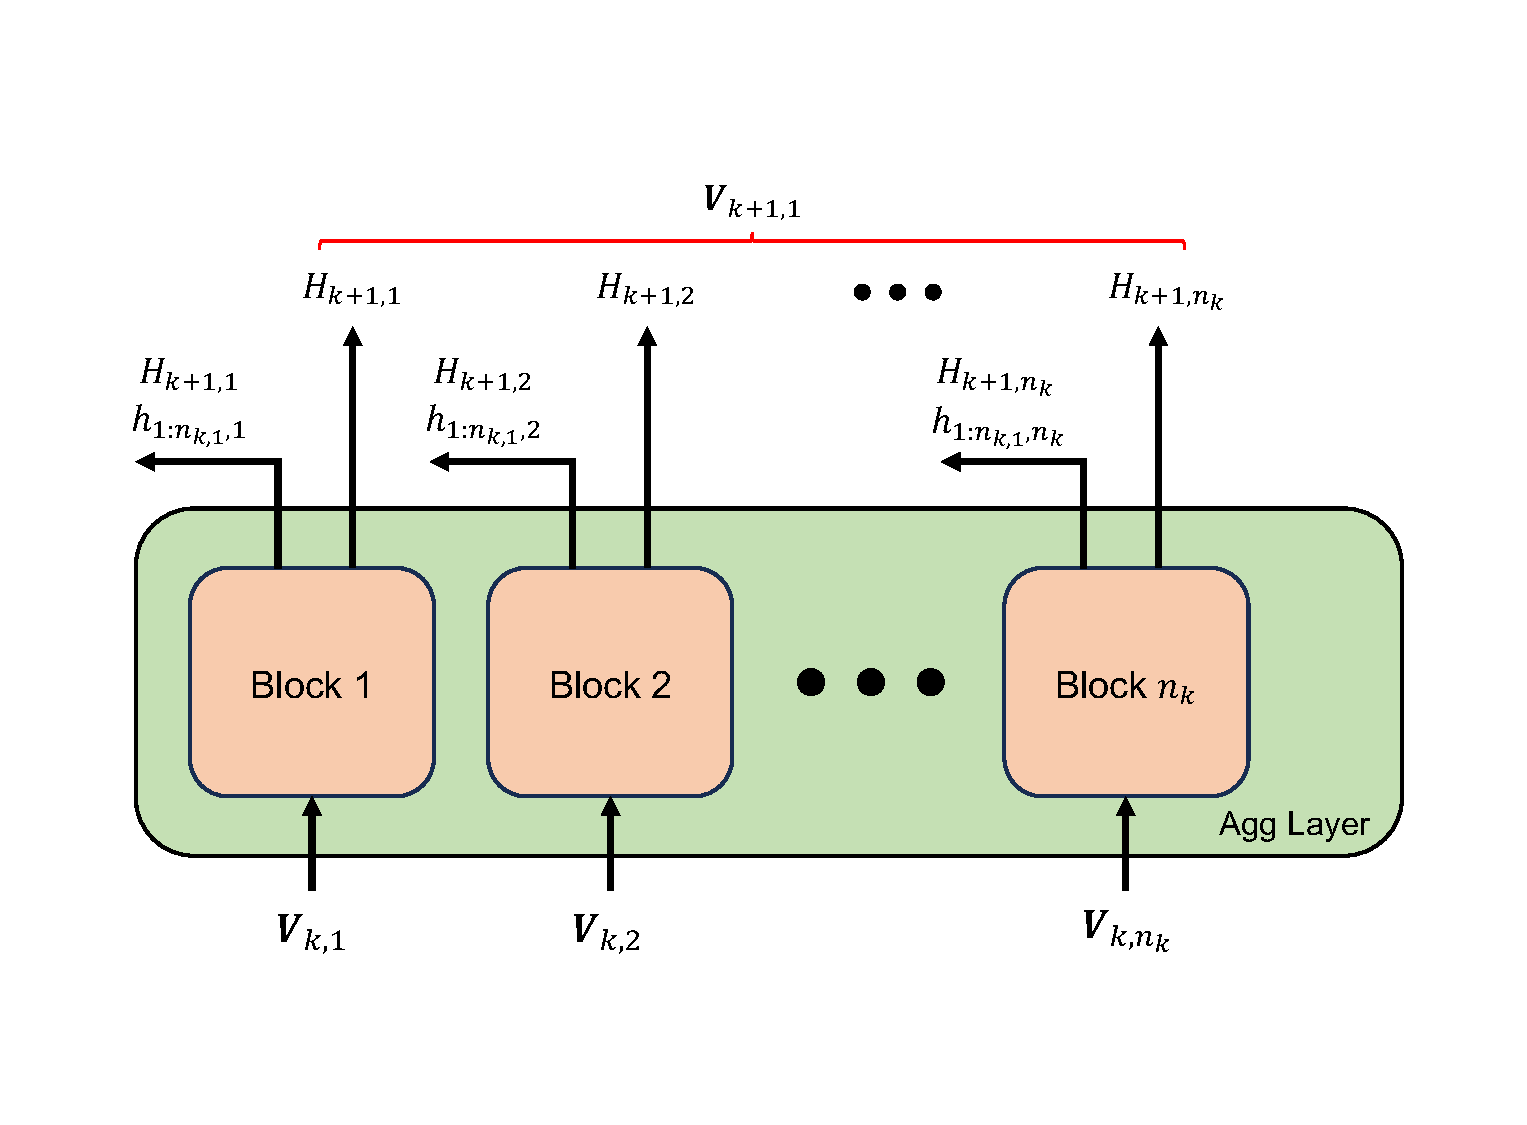
\includegraphics[trim=0.7cm 1.2cm 0.9cm 1.2cm, width=0.93\linewidth]{Contents/img/layer.pdf}
    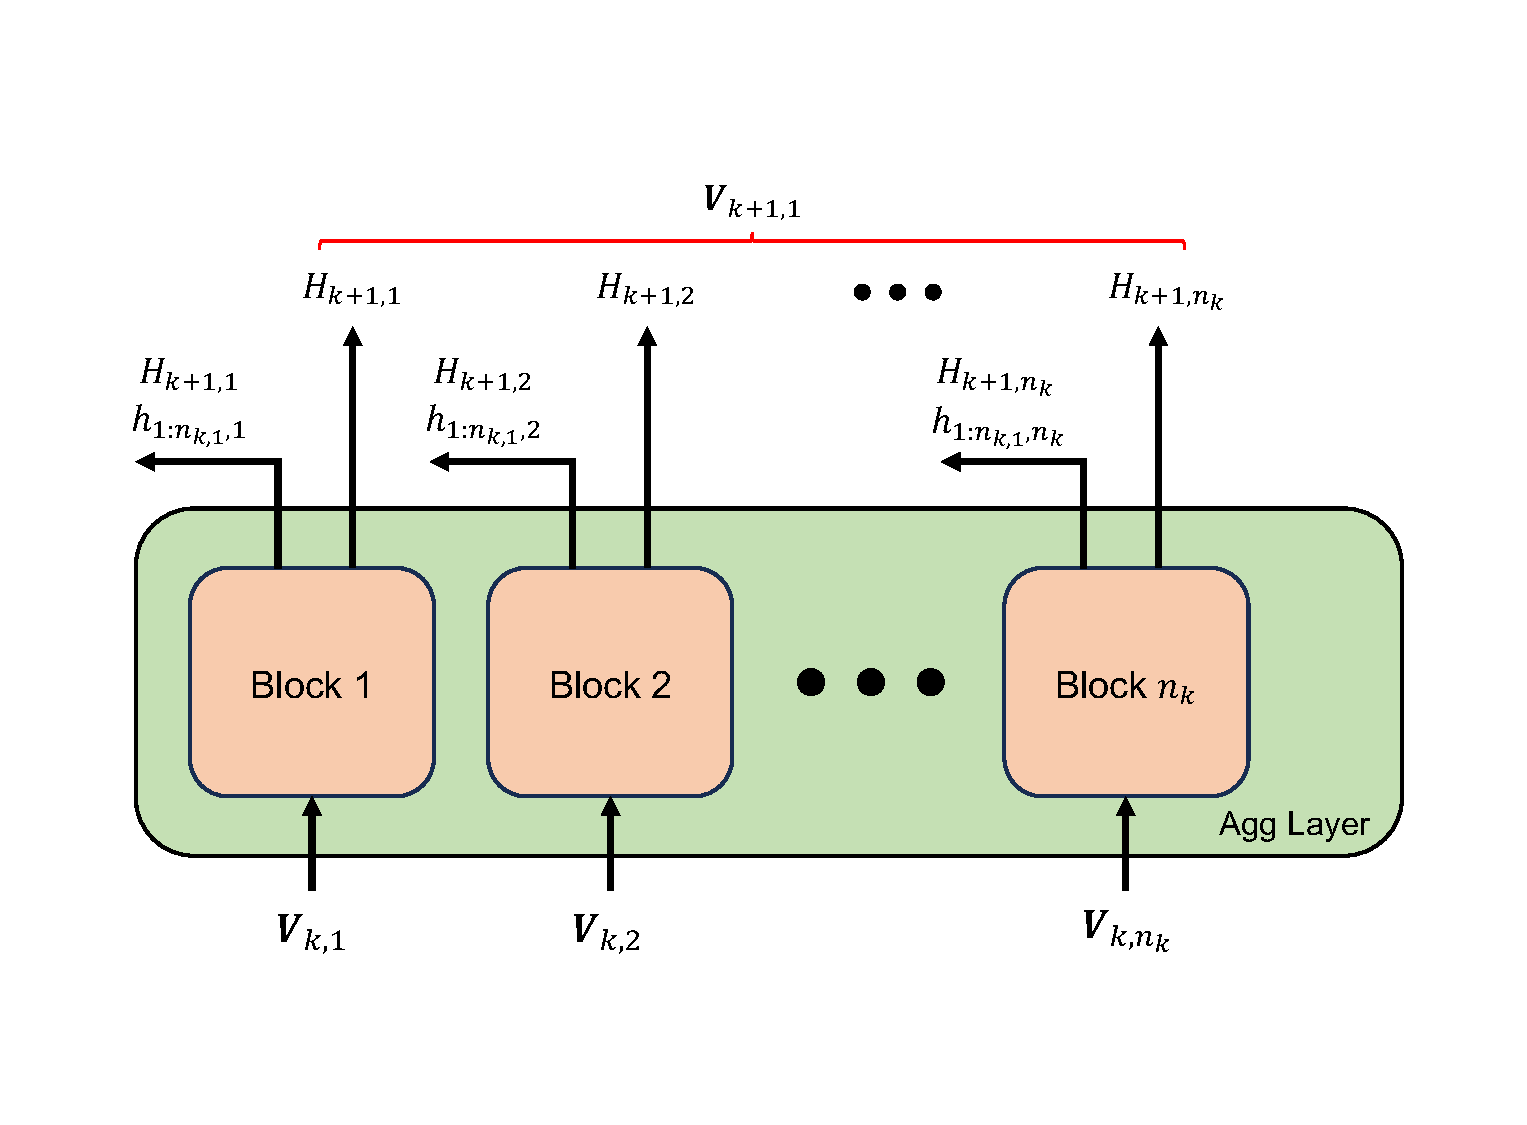
\includegraphics[trim=0.7cm 1.7cm 0.9cm 1.4cm, scale=0.3]{Contents/img/layer.pdf}
    \caption{The inner structure of an aggregation layer.}
    \label{layer}
\end{figure}

\paragraph{Semantics Refinement}
In the lower layer where the feature scale is small and dense, there are closed semantic units, which result in many duplicated matching scores and impair the ability of prediction network (as we show in the next section)
To address this problem, we aim to filter the extremely long sequences of output features, only to maintain the dominant components.
The algorithm is based on a faster $k$-means algorithm, which can produce a set of representations by clustering adjacent points so that redundant semantics are eliminated.
To reduce extra overhead, we implement an approximate but faster algorithm~\cite{hamerly2010making}~only when the feature number exceeds a threshold.
To prevent each clustered set from being too small (i.e., only 1 or 2 points) and ensure efficiency, we random sample $C$ points as centers.
The algorithm is formally depicted in~\Cref{alg:1}, where we omit the specific steps of fast $k$-means and readers can refer to the paper~\cite{hamerly2010making} for the details. It should be emphasized that $k$-means is a non-parametric clustering algorithm and only incurs negligible overhead in the forward pass.
\begin{algorithm}[h!]
    \small
    \SetKwFunction{ret}{return}
    \SetKwFunction{RS}{RandomSample}
    \SetKwFunction{RI}{RandomInit}
    \SetKwFunction{KM}{$k$-Means}
    \SetAlgoLined
    \KwIn{Semantic elements set $S=\{s_1,s_2,...,s_N\}$, expected cluster size $r$, number of centers $C$, }
    \KwOut{Refined set $S'=\{s'_1,s'_2,...,s'_{C}\}$}
    \BlankLine
    \uIf{$N \leq C \times r$}
    {\ret \RS$(S,C)$ \\
    }\Else{
        \ret $\KM(\RI(C),S)$ \\
    }
\caption{\textbf{Semantics Refinement}}
\label{alg:1}
\end{algorithm}

In the algorithm, $C$ bounds the lowest number of centers required for the later computation and a typical value could be $C=\lceil \sqrt{K} \rceil$ where $K$ is the hyperparameter in the last layer's feature selector (as stated below) implicitly and roughly. The heuristics in using squareroot comes from the fact that similarity scores are computed in pair. 
Here $r$ is another important hyperparameter that controls the expected (or average) cluster size to avoid overmuch small clusters.

\paragraph{Prediction} After obtaining the representations from both fields and modalities in all scales ($H_k, h_{1:n_k}$), we concatenate them into four matrices $\mathbf{R}^{t,p},\mathbf{R}^{t,r},\mathbf{R}^{v,p},\mathbf{R}^{v, r}$ whose rows are these representation vectors.
Concretely, we extract the n-gram token, sentence, and n-gram sentence representations for text, and n-gram RoI and image representations for the image.
We hypothesize that the review quality depends on the semantic coherence existing within 
1) The image-text pair in the review to guarantee the coherence of the review itself. Low-quality reviews are usually not self-contained ($\mathbf{R}^{t,r},\mathbf{R}^{v,r}$). 
We exclude the scores of image-text pairs from product introduction because they do not have any impact to the helpfulness of a review.
2) The same modality from different fields ($\mathbf{R}^{t,p},\mathbf{R}^{t,r}$ and $\mathbf{R}^{v,p},\mathbf{R}^{v,r}$). This is important because user-preferred comments should directly response to the selling points in the introduction.

The matching scores are calculated as the cosine similarities between row vectors of two matrices:
\begin{equation}
    \label{eq:cos_sim}
    \textbf{S}(\mathbf{A},\mathbf{B}) = \mathbf{cosine}(\mathbf{A},\mathbf{B}) = \frac{\mathbf{A}\mathbf{B}^T}{\Vert \mathbf{A} \Vert\cdot\Vert \mathbf{B} \Vert^T} \\
\end{equation}
where $\Vert \cdot \Vert$ is the row-wise L2 normalization.
Suppose there are $n_1,n_2,n_3,n_4$ rows (the number of feature vectors) in the four matrices, then we have $n_1n_2+n_2n_4+n_3n_4$ matching scores.
We then picked the highest $K$ scores to form the last features. 
It should be emphasized that the top-K operation reorganizes the tensors during its computation. 
\begin{equation}
    \mathbf{h} = \mathbf{TopK}(\mathbf{FlattenAll}(\mathbf{S'}))
\end{equation}
Therefore the gradient back-propagation path is not constant given different input samples. The predictions for training and inference are calculated from the feature:
\begin{equation}
    \mathbf{f}_{i,j} = \sigma(\mathrm{Linear}(\mathbf{h}_{i,j}))
\end{equation}
where $\sigma$ is the Sigmoid function.

\subsection{Training}
\label{sec:Training}
We follow \citet{nguyen2023gradient}~to apply the listwise loss for training.
\begin{equation}
    \mathcal{L} = -\sum_{i=1}^{\vert P \vert}\sum_{j=1}^{\vert R_i \vert}y_{i,j}'\log(f_{i,j}')
\end{equation}
where $\vert \mathcal{P} \vert$ is the number of productions in the batch and $\vert R_i \vert$ is the number of reviews corresponding to $P_i$. The normalized labels $y'$ and predictions $f'$ are given by
\begin{equation}
    f'_{i,j} = \mathrm{softmax}(\mathbf{f}_i)_j,
    y'_{i,j} = \mathrm{softmax}(\mathbf{y}_i)_j
\end{equation}
Note that the final predictions are ranged within $(0, 1)$, which diverges from the true label distribution $y \in [0,4]$. However, the ultimate target (same as the evaluation metrics) of the task concentrates on \textit{ranking} (relative value) rather than absolute value. This kind of learning can still benefit the performance.
